% Graphic for TeX using PGF
% Title: C:\Documents and Settings\antoine.deroquemaure\Mes documents\stage\rapport\images\2-activite\DiagrammeClassServer.dia
% Creator: Dia v0.97.2
% CreationDate: Mon Jun 11 18:51:01 2012
% For: antoine.deroquemaure
% \usepackage{tikz}
% The following commands are not supported in PSTricks at present
% We define them conditionally, so when they are implemented,
% this pgf file will use them.
\ifx\du\undefined
  \newlength{\du}
\fi
\setlength{\du}{15\unitlength}
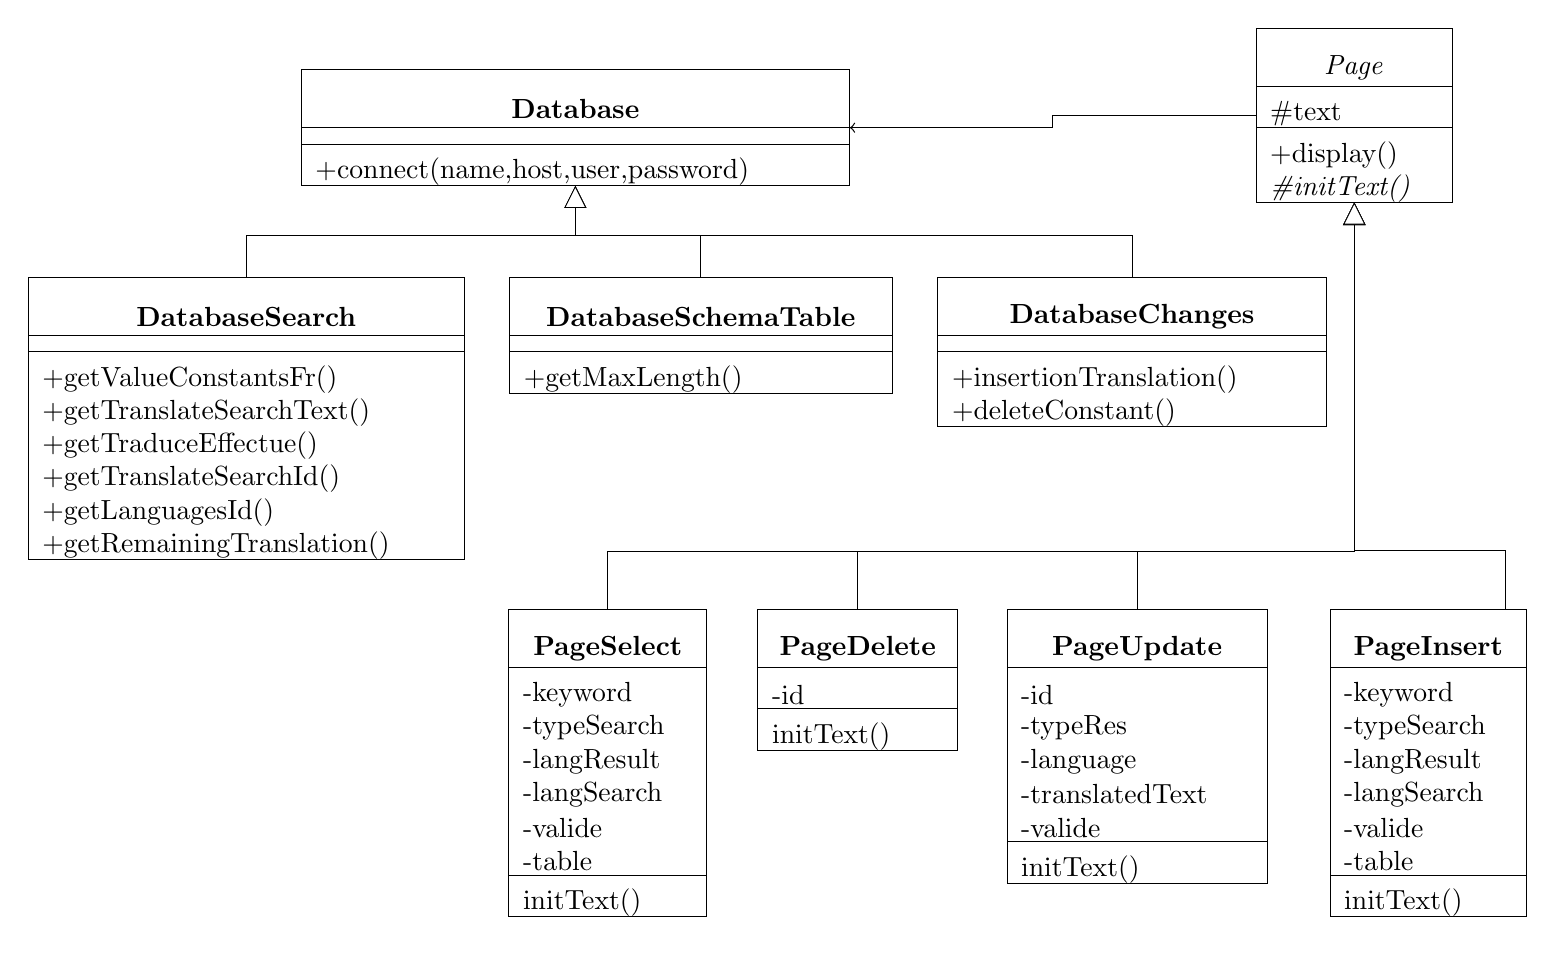
\begin{tikzpicture}
\pgftransformxscale{1.000000}
\pgftransformyscale{-1.000000}
\definecolor{dialinecolor}{rgb}{0.000000, 0.000000, 0.000000}
\pgfsetstrokecolor{dialinecolor}
\definecolor{dialinecolor}{rgb}{1.000000, 1.000000, 1.000000}
\pgfsetfillcolor{dialinecolor}
\pgfsetlinewidth{0.020000\du}
\pgfsetdash{}{0pt}
\definecolor{dialinecolor}{rgb}{1.000000, 1.000000, 1.000000}
\pgfsetfillcolor{dialinecolor}
\fill (-12.000000\du,0.000000\du)--(-12.000000\du,1.400000\du)--(-7.265000\du,1.400000\du)--(-7.265000\du,0.000000\du)--cycle;
\definecolor{dialinecolor}{rgb}{0.000000, 0.000000, 0.000000}
\pgfsetstrokecolor{dialinecolor}
\draw (-12.000000\du,0.000000\du)--(-12.000000\du,1.400000\du)--(-7.265000\du,1.400000\du)--(-7.265000\du,0.000000\du)--cycle;
% setfont left to latex
\definecolor{dialinecolor}{rgb}{0.000000, 0.000000, 0.000000}
\pgfsetstrokecolor{dialinecolor}
\node at (-9.632500\du,0.950000\du){\textit{Page}};
\definecolor{dialinecolor}{rgb}{1.000000, 1.000000, 1.000000}
\pgfsetfillcolor{dialinecolor}
\fill (-12.000000\du,1.400000\du)--(-12.000000\du,2.400000\du)--(-7.265000\du,2.400000\du)--(-7.265000\du,1.400000\du)--cycle;
\definecolor{dialinecolor}{rgb}{0.000000, 0.000000, 0.000000}
\pgfsetstrokecolor{dialinecolor}
\draw (-12.000000\du,1.400000\du)--(-12.000000\du,2.400000\du)--(-7.265000\du,2.400000\du)--(-7.265000\du,1.400000\du)--cycle;
% setfont left to latex
\definecolor{dialinecolor}{rgb}{0.000000, 0.000000, 0.000000}
\pgfsetstrokecolor{dialinecolor}
\node[anchor=west] at (-11.890000\du,2.060000\du){\#text};
\definecolor{dialinecolor}{rgb}{1.000000, 1.000000, 1.000000}
\pgfsetfillcolor{dialinecolor}
\fill (-12.000000\du,2.400000\du)--(-12.000000\du,4.200000\du)--(-7.265000\du,4.200000\du)--(-7.265000\du,2.400000\du)--cycle;
\definecolor{dialinecolor}{rgb}{0.000000, 0.000000, 0.000000}
\pgfsetstrokecolor{dialinecolor}
\draw (-12.000000\du,2.400000\du)--(-12.000000\du,4.200000\du)--(-7.265000\du,4.200000\du)--(-7.265000\du,2.400000\du)--cycle;
% setfont left to latex
\definecolor{dialinecolor}{rgb}{0.000000, 0.000000, 0.000000}
\pgfsetstrokecolor{dialinecolor}
\node[anchor=west] at (-11.890000\du,3.060000\du){+display()};
% setfont left to latex
\definecolor{dialinecolor}{rgb}{0.000000, 0.000000, 0.000000}
\pgfsetstrokecolor{dialinecolor}
\node[anchor=west] at (-11.890000\du,3.860000\du){\textit{\#initText()}};
\pgfsetlinewidth{0.020000\du}
\pgfsetdash{}{0pt}
\definecolor{dialinecolor}{rgb}{1.000000, 1.000000, 1.000000}
\pgfsetfillcolor{dialinecolor}
\fill (-30.000000\du,14.000000\du)--(-30.000000\du,15.400000\du)--(-25.232500\du,15.400000\du)--(-25.232500\du,14.000000\du)--cycle;
\definecolor{dialinecolor}{rgb}{0.000000, 0.000000, 0.000000}
\pgfsetstrokecolor{dialinecolor}
\draw (-30.000000\du,14.000000\du)--(-30.000000\du,15.400000\du)--(-25.232500\du,15.400000\du)--(-25.232500\du,14.000000\du)--cycle;
% setfont left to latex
\definecolor{dialinecolor}{rgb}{0.000000, 0.000000, 0.000000}
\pgfsetstrokecolor{dialinecolor}
\node at (-27.616250\du,14.950000\du){\textbf{PageSelect}};
\definecolor{dialinecolor}{rgb}{1.000000, 1.000000, 1.000000}
\pgfsetfillcolor{dialinecolor}
\fill (-30.000000\du,15.400000\du)--(-30.000000\du,20.400000\du)--(-25.232500\du,20.400000\du)--(-25.232500\du,15.400000\du)--cycle;
\definecolor{dialinecolor}{rgb}{0.000000, 0.000000, 0.000000}
\pgfsetstrokecolor{dialinecolor}
\draw (-30.000000\du,15.400000\du)--(-30.000000\du,20.400000\du)--(-25.232500\du,20.400000\du)--(-25.232500\du,15.400000\du)--cycle;
% setfont left to latex
\definecolor{dialinecolor}{rgb}{0.000000, 0.000000, 0.000000}
\pgfsetstrokecolor{dialinecolor}
\node[anchor=west] at (-29.890000\du,16.060000\du){-keyword};
% setfont left to latex
\definecolor{dialinecolor}{rgb}{0.000000, 0.000000, 0.000000}
\pgfsetstrokecolor{dialinecolor}
\node[anchor=west] at (-29.890000\du,16.860000\du){-typeSearch};
% setfont left to latex
\definecolor{dialinecolor}{rgb}{0.000000, 0.000000, 0.000000}
\pgfsetstrokecolor{dialinecolor}
\node[anchor=west] at (-29.890000\du,17.660000\du){-langResult};
% setfont left to latex
\definecolor{dialinecolor}{rgb}{0.000000, 0.000000, 0.000000}
\pgfsetstrokecolor{dialinecolor}
\node[anchor=west] at (-29.890000\du,18.460000\du){-langSearch};
% setfont left to latex
\definecolor{dialinecolor}{rgb}{0.000000, 0.000000, 0.000000}
\pgfsetstrokecolor{dialinecolor}
\node[anchor=west] at (-29.890000\du,19.260000\du){-valide};
% setfont left to latex
\definecolor{dialinecolor}{rgb}{0.000000, 0.000000, 0.000000}
\pgfsetstrokecolor{dialinecolor}
\node[anchor=west] at (-29.890000\du,20.060000\du){-table};
\definecolor{dialinecolor}{rgb}{1.000000, 1.000000, 1.000000}
\pgfsetfillcolor{dialinecolor}
\fill (-30.000000\du,20.400000\du)--(-30.000000\du,21.400000\du)--(-25.232500\du,21.400000\du)--(-25.232500\du,20.400000\du)--cycle;
\definecolor{dialinecolor}{rgb}{0.000000, 0.000000, 0.000000}
\pgfsetstrokecolor{dialinecolor}
\draw (-30.000000\du,20.400000\du)--(-30.000000\du,21.400000\du)--(-25.232500\du,21.400000\du)--(-25.232500\du,20.400000\du)--cycle;
% setfont left to latex
\definecolor{dialinecolor}{rgb}{0.000000, 0.000000, 0.000000}
\pgfsetstrokecolor{dialinecolor}
\node[anchor=west] at (-29.890000\du,21.060000\du){ initText()};
\pgfsetlinewidth{0.020000\du}
\pgfsetdash{}{0pt}
\definecolor{dialinecolor}{rgb}{1.000000, 1.000000, 1.000000}
\pgfsetfillcolor{dialinecolor}
\fill (-24.000000\du,14.000000\du)--(-24.000000\du,15.400000\du)--(-19.187500\du,15.400000\du)--(-19.187500\du,14.000000\du)--cycle;
\definecolor{dialinecolor}{rgb}{0.000000, 0.000000, 0.000000}
\pgfsetstrokecolor{dialinecolor}
\draw (-24.000000\du,14.000000\du)--(-24.000000\du,15.400000\du)--(-19.187500\du,15.400000\du)--(-19.187500\du,14.000000\du)--cycle;
% setfont left to latex
\definecolor{dialinecolor}{rgb}{0.000000, 0.000000, 0.000000}
\pgfsetstrokecolor{dialinecolor}
\node at (-21.593750\du,14.950000\du){\textbf{PageDelete}};
\definecolor{dialinecolor}{rgb}{1.000000, 1.000000, 1.000000}
\pgfsetfillcolor{dialinecolor}
\fill (-24.000000\du,15.400000\du)--(-24.000000\du,16.400000\du)--(-19.187500\du,16.400000\du)--(-19.187500\du,15.400000\du)--cycle;
\definecolor{dialinecolor}{rgb}{0.000000, 0.000000, 0.000000}
\pgfsetstrokecolor{dialinecolor}
\draw (-24.000000\du,15.400000\du)--(-24.000000\du,16.400000\du)--(-19.187500\du,16.400000\du)--(-19.187500\du,15.400000\du)--cycle;
% setfont left to latex
\definecolor{dialinecolor}{rgb}{0.000000, 0.000000, 0.000000}
\pgfsetstrokecolor{dialinecolor}
\node[anchor=west] at (-23.890000\du,16.060000\du){-id};
\definecolor{dialinecolor}{rgb}{1.000000, 1.000000, 1.000000}
\pgfsetfillcolor{dialinecolor}
\fill (-24.000000\du,16.400000\du)--(-24.000000\du,17.400000\du)--(-19.187500\du,17.400000\du)--(-19.187500\du,16.400000\du)--cycle;
\definecolor{dialinecolor}{rgb}{0.000000, 0.000000, 0.000000}
\pgfsetstrokecolor{dialinecolor}
\draw (-24.000000\du,16.400000\du)--(-24.000000\du,17.400000\du)--(-19.187500\du,17.400000\du)--(-19.187500\du,16.400000\du)--cycle;
% setfont left to latex
\definecolor{dialinecolor}{rgb}{0.000000, 0.000000, 0.000000}
\pgfsetstrokecolor{dialinecolor}
\node[anchor=west] at (-23.890000\du,17.060000\du){ initText()};
\pgfsetlinewidth{0.020000\du}
\pgfsetdash{}{0pt}
\definecolor{dialinecolor}{rgb}{1.000000, 1.000000, 1.000000}
\pgfsetfillcolor{dialinecolor}
\fill (-18.000000\du,14.000000\du)--(-18.000000\du,15.400000\du)--(-11.725000\du,15.400000\du)--(-11.725000\du,14.000000\du)--cycle;
\definecolor{dialinecolor}{rgb}{0.000000, 0.000000, 0.000000}
\pgfsetstrokecolor{dialinecolor}
\draw (-18.000000\du,14.000000\du)--(-18.000000\du,15.400000\du)--(-11.725000\du,15.400000\du)--(-11.725000\du,14.000000\du)--cycle;
% setfont left to latex
\definecolor{dialinecolor}{rgb}{0.000000, 0.000000, 0.000000}
\pgfsetstrokecolor{dialinecolor}
\node at (-14.862500\du,14.950000\du){\textbf{PageUpdate}};
\definecolor{dialinecolor}{rgb}{1.000000, 1.000000, 1.000000}
\pgfsetfillcolor{dialinecolor}
\fill (-18.000000\du,15.400000\du)--(-18.000000\du,19.600000\du)--(-11.725000\du,19.600000\du)--(-11.725000\du,15.400000\du)--cycle;
\definecolor{dialinecolor}{rgb}{0.000000, 0.000000, 0.000000}
\pgfsetstrokecolor{dialinecolor}
\draw (-18.000000\du,15.400000\du)--(-18.000000\du,19.600000\du)--(-11.725000\du,19.600000\du)--(-11.725000\du,15.400000\du)--cycle;
% setfont left to latex
\definecolor{dialinecolor}{rgb}{0.000000, 0.000000, 0.000000}
\pgfsetstrokecolor{dialinecolor}
\node[anchor=west] at (-17.890000\du,16.060000\du){-id};
% setfont left to latex
\definecolor{dialinecolor}{rgb}{0.000000, 0.000000, 0.000000}
\pgfsetstrokecolor{dialinecolor}
\node[anchor=west] at (-17.890000\du,16.860000\du){-typeRes};
% setfont left to latex
\definecolor{dialinecolor}{rgb}{0.000000, 0.000000, 0.000000}
\pgfsetstrokecolor{dialinecolor}
\node[anchor=west] at (-17.890000\du,17.660000\du){-language};
% setfont left to latex
\definecolor{dialinecolor}{rgb}{0.000000, 0.000000, 0.000000}
\pgfsetstrokecolor{dialinecolor}
\node[anchor=west] at (-17.890000\du,18.460000\du){-translatedText};
% setfont left to latex
\definecolor{dialinecolor}{rgb}{0.000000, 0.000000, 0.000000}
\pgfsetstrokecolor{dialinecolor}
\node[anchor=west] at (-17.890000\du,19.260000\du){-valide};
\definecolor{dialinecolor}{rgb}{1.000000, 1.000000, 1.000000}
\pgfsetfillcolor{dialinecolor}
\fill (-18.000000\du,19.600000\du)--(-18.000000\du,20.600000\du)--(-11.725000\du,20.600000\du)--(-11.725000\du,19.600000\du)--cycle;
\definecolor{dialinecolor}{rgb}{0.000000, 0.000000, 0.000000}
\pgfsetstrokecolor{dialinecolor}
\draw (-18.000000\du,19.600000\du)--(-18.000000\du,20.600000\du)--(-11.725000\du,20.600000\du)--(-11.725000\du,19.600000\du)--cycle;
% setfont left to latex
\definecolor{dialinecolor}{rgb}{0.000000, 0.000000, 0.000000}
\pgfsetstrokecolor{dialinecolor}
\node[anchor=west] at (-17.890000\du,20.260000\du){ initText()};
\pgfsetlinewidth{0.030000\du}
\pgfsetdash{}{0pt}
\pgfsetdash{}{0pt}
\pgfsetmiterjoin
\pgfsetbuttcap
{
\definecolor{dialinecolor}{rgb}{0.000000, 0.000000, 0.000000}
\pgfsetfillcolor{dialinecolor}
% was here!!!
{\pgfsetcornersarced{\pgfpoint{0.000000\du}{0.000000\du}}\definecolor{dialinecolor}{rgb}{0.000000, 0.000000, 0.000000}
\pgfsetstrokecolor{dialinecolor}
\draw (-27.616250\du,14.000000\du)--(-27.616250\du,12.600000\du)--(-9.632500\du,12.600000\du)--(-9.632500\du,4.200000\du);
}}
{\pgfsetcornersarced{\pgfpoint{0.000000\du}{0.000000\du}}\definecolor{dialinecolor}{rgb}{0.000000, 0.000000, 0.000000}
\pgfsetstrokecolor{dialinecolor}
\draw (-27.616250\du,14.000000\du)--(-27.616250\du,12.600000\du)--(-9.632500\du,12.600000\du)--(-9.632500\du,4.733541\du);
}\pgfsetmiterjoin
\definecolor{dialinecolor}{rgb}{1.000000, 1.000000, 1.000000}
\pgfsetfillcolor{dialinecolor}
\fill (-9.382500\du,4.733541\du)--(-9.632500\du,4.233541\du)--(-9.882500\du,4.733541\du)--cycle;
\pgfsetlinewidth{0.030000\du}
\pgfsetdash{}{0pt}
\pgfsetmiterjoin
\definecolor{dialinecolor}{rgb}{0.000000, 0.000000, 0.000000}
\pgfsetstrokecolor{dialinecolor}
\draw (-9.382500\du,4.733541\du)--(-9.632500\du,4.233541\du)--(-9.882500\du,4.733541\du)--cycle;
\pgfsetlinewidth{0.030000\du}
\pgfsetdash{}{0pt}
\pgfsetdash{}{0pt}
\pgfsetmiterjoin
\pgfsetbuttcap
{
\definecolor{dialinecolor}{rgb}{0.000000, 0.000000, 0.000000}
\pgfsetfillcolor{dialinecolor}
% was here!!!
{\pgfsetcornersarced{\pgfpoint{0.000000\du}{0.000000\du}}\definecolor{dialinecolor}{rgb}{0.000000, 0.000000, 0.000000}
\pgfsetstrokecolor{dialinecolor}
\draw (-21.593750\du,14.000000\du)--(-21.593750\du,12.600000\du)--(-9.632500\du,12.600000\du)--(-9.632500\du,4.200000\du);
}}
{\pgfsetcornersarced{\pgfpoint{0.000000\du}{0.000000\du}}\definecolor{dialinecolor}{rgb}{0.000000, 0.000000, 0.000000}
\pgfsetstrokecolor{dialinecolor}
\draw (-21.593750\du,14.000000\du)--(-21.593750\du,12.600000\du)--(-9.632500\du,12.600000\du)--(-9.632500\du,4.733541\du);
}\pgfsetmiterjoin
\definecolor{dialinecolor}{rgb}{1.000000, 1.000000, 1.000000}
\pgfsetfillcolor{dialinecolor}
\fill (-9.382500\du,4.733541\du)--(-9.632500\du,4.233541\du)--(-9.882500\du,4.733541\du)--cycle;
\pgfsetlinewidth{0.030000\du}
\pgfsetdash{}{0pt}
\pgfsetmiterjoin
\definecolor{dialinecolor}{rgb}{0.000000, 0.000000, 0.000000}
\pgfsetstrokecolor{dialinecolor}
\draw (-9.382500\du,4.733541\du)--(-9.632500\du,4.233541\du)--(-9.882500\du,4.733541\du)--cycle;
\pgfsetlinewidth{0.030000\du}
\pgfsetdash{}{0pt}
\pgfsetdash{}{0pt}
\pgfsetmiterjoin
\pgfsetbuttcap
{
\definecolor{dialinecolor}{rgb}{0.000000, 0.000000, 0.000000}
\pgfsetfillcolor{dialinecolor}
% was here!!!
{\pgfsetcornersarced{\pgfpoint{0.000000\du}{0.000000\du}}\definecolor{dialinecolor}{rgb}{0.000000, 0.000000, 0.000000}
\pgfsetstrokecolor{dialinecolor}
\draw (-14.862500\du,14.000000\du)--(-14.862500\du,12.600000\du)--(-9.632500\du,12.600000\du)--(-9.632500\du,4.200000\du);
}}
{\pgfsetcornersarced{\pgfpoint{0.000000\du}{0.000000\du}}\definecolor{dialinecolor}{rgb}{0.000000, 0.000000, 0.000000}
\pgfsetstrokecolor{dialinecolor}
\draw (-14.862500\du,14.000000\du)--(-14.862500\du,12.600000\du)--(-9.632500\du,12.600000\du)--(-9.632500\du,4.733541\du);
}\pgfsetmiterjoin
\definecolor{dialinecolor}{rgb}{1.000000, 1.000000, 1.000000}
\pgfsetfillcolor{dialinecolor}
\fill (-9.382500\du,4.733541\du)--(-9.632500\du,4.233541\du)--(-9.882500\du,4.733541\du)--cycle;
\pgfsetlinewidth{0.030000\du}
\pgfsetdash{}{0pt}
\pgfsetmiterjoin
\definecolor{dialinecolor}{rgb}{0.000000, 0.000000, 0.000000}
\pgfsetstrokecolor{dialinecolor}
\draw (-9.382500\du,4.733541\du)--(-9.632500\du,4.233541\du)--(-9.882500\du,4.733541\du)--cycle;
\pgfsetlinewidth{0.020000\du}
\pgfsetdash{}{0pt}
\definecolor{dialinecolor}{rgb}{1.000000, 1.000000, 1.000000}
\pgfsetfillcolor{dialinecolor}
\fill (-35.000000\du,1.000000\du)--(-35.000000\du,2.400000\du)--(-21.795000\du,2.400000\du)--(-21.795000\du,1.000000\du)--cycle;
\definecolor{dialinecolor}{rgb}{0.000000, 0.000000, 0.000000}
\pgfsetstrokecolor{dialinecolor}
\draw (-35.000000\du,1.000000\du)--(-35.000000\du,2.400000\du)--(-21.795000\du,2.400000\du)--(-21.795000\du,1.000000\du)--cycle;
% setfont left to latex
\definecolor{dialinecolor}{rgb}{0.000000, 0.000000, 0.000000}
\pgfsetstrokecolor{dialinecolor}
\node at (-28.397500\du,1.950000\du){\textbf{Database}};
\definecolor{dialinecolor}{rgb}{1.000000, 1.000000, 1.000000}
\pgfsetfillcolor{dialinecolor}
\fill (-35.000000\du,2.400000\du)--(-35.000000\du,2.800000\du)--(-21.795000\du,2.800000\du)--(-21.795000\du,2.400000\du)--cycle;
\definecolor{dialinecolor}{rgb}{0.000000, 0.000000, 0.000000}
\pgfsetstrokecolor{dialinecolor}
\draw (-35.000000\du,2.400000\du)--(-35.000000\du,2.800000\du)--(-21.795000\du,2.800000\du)--(-21.795000\du,2.400000\du)--cycle;
\definecolor{dialinecolor}{rgb}{1.000000, 1.000000, 1.000000}
\pgfsetfillcolor{dialinecolor}
\fill (-35.000000\du,2.800000\du)--(-35.000000\du,3.800000\du)--(-21.795000\du,3.800000\du)--(-21.795000\du,2.800000\du)--cycle;
\definecolor{dialinecolor}{rgb}{0.000000, 0.000000, 0.000000}
\pgfsetstrokecolor{dialinecolor}
\draw (-35.000000\du,2.800000\du)--(-35.000000\du,3.800000\du)--(-21.795000\du,3.800000\du)--(-21.795000\du,2.800000\du)--cycle;
% setfont left to latex
\definecolor{dialinecolor}{rgb}{0.000000, 0.000000, 0.000000}
\pgfsetstrokecolor{dialinecolor}
\node[anchor=west] at (-34.890000\du,3.460000\du){+connect(name,host,user,password)};
\pgfsetlinewidth{0.020000\du}
\pgfsetdash{}{0pt}
\definecolor{dialinecolor}{rgb}{1.000000, 1.000000, 1.000000}
\pgfsetfillcolor{dialinecolor}
\fill (-10.218100\du,14.000000\du)--(-10.218100\du,15.400000\du)--(-5.483100\du,15.400000\du)--(-5.483100\du,14.000000\du)--cycle;
\definecolor{dialinecolor}{rgb}{0.000000, 0.000000, 0.000000}
\pgfsetstrokecolor{dialinecolor}
\draw (-10.218100\du,14.000000\du)--(-10.218100\du,15.400000\du)--(-5.483100\du,15.400000\du)--(-5.483100\du,14.000000\du)--cycle;
% setfont left to latex
\definecolor{dialinecolor}{rgb}{0.000000, 0.000000, 0.000000}
\pgfsetstrokecolor{dialinecolor}
\node at (-7.850600\du,14.950000\du){\textbf{PageInsert}};
\definecolor{dialinecolor}{rgb}{1.000000, 1.000000, 1.000000}
\pgfsetfillcolor{dialinecolor}
\fill (-10.218100\du,15.400000\du)--(-10.218100\du,20.400000\du)--(-5.483100\du,20.400000\du)--(-5.483100\du,15.400000\du)--cycle;
\definecolor{dialinecolor}{rgb}{0.000000, 0.000000, 0.000000}
\pgfsetstrokecolor{dialinecolor}
\draw (-10.218100\du,15.400000\du)--(-10.218100\du,20.400000\du)--(-5.483100\du,20.400000\du)--(-5.483100\du,15.400000\du)--cycle;
% setfont left to latex
\definecolor{dialinecolor}{rgb}{0.000000, 0.000000, 0.000000}
\pgfsetstrokecolor{dialinecolor}
\node[anchor=west] at (-10.108100\du,16.060000\du){-keyword};
% setfont left to latex
\definecolor{dialinecolor}{rgb}{0.000000, 0.000000, 0.000000}
\pgfsetstrokecolor{dialinecolor}
\node[anchor=west] at (-10.108100\du,16.860000\du){-typeSearch};
% setfont left to latex
\definecolor{dialinecolor}{rgb}{0.000000, 0.000000, 0.000000}
\pgfsetstrokecolor{dialinecolor}
\node[anchor=west] at (-10.108100\du,17.660000\du){-langResult};
% setfont left to latex
\definecolor{dialinecolor}{rgb}{0.000000, 0.000000, 0.000000}
\pgfsetstrokecolor{dialinecolor}
\node[anchor=west] at (-10.108100\du,18.460000\du){-langSearch};
% setfont left to latex
\definecolor{dialinecolor}{rgb}{0.000000, 0.000000, 0.000000}
\pgfsetstrokecolor{dialinecolor}
\node[anchor=west] at (-10.108100\du,19.260000\du){-valide};
% setfont left to latex
\definecolor{dialinecolor}{rgb}{0.000000, 0.000000, 0.000000}
\pgfsetstrokecolor{dialinecolor}
\node[anchor=west] at (-10.108100\du,20.060000\du){-table};
\definecolor{dialinecolor}{rgb}{1.000000, 1.000000, 1.000000}
\pgfsetfillcolor{dialinecolor}
\fill (-10.218100\du,20.400000\du)--(-10.218100\du,21.400000\du)--(-5.483100\du,21.400000\du)--(-5.483100\du,20.400000\du)--cycle;
\definecolor{dialinecolor}{rgb}{0.000000, 0.000000, 0.000000}
\pgfsetstrokecolor{dialinecolor}
\draw (-10.218100\du,20.400000\du)--(-10.218100\du,21.400000\du)--(-5.483100\du,21.400000\du)--(-5.483100\du,20.400000\du)--cycle;
% setfont left to latex
\definecolor{dialinecolor}{rgb}{0.000000, 0.000000, 0.000000}
\pgfsetstrokecolor{dialinecolor}
\node[anchor=west] at (-10.108100\du,21.060000\du){ initText()};
\pgfsetlinewidth{0.030000\du}
\pgfsetdash{}{0pt}
\pgfsetdash{}{0pt}
\pgfsetmiterjoin
\pgfsetbuttcap
{
\definecolor{dialinecolor}{rgb}{0.000000, 0.000000, 0.000000}
\pgfsetfillcolor{dialinecolor}
% was here!!!
\pgfsetarrowsend{to}
{\pgfsetcornersarced{\pgfpoint{0.000000\du}{0.000000\du}}\definecolor{dialinecolor}{rgb}{0.000000, 0.000000, 0.000000}
\pgfsetstrokecolor{dialinecolor}
\draw (-12.010290\du,2.100000\du)--(-16.897443\du,2.100000\du)--(-16.897443\du,2.400000\du)--(-21.784596\du,2.400000\du);
}}
\pgfsetlinewidth{0.020000\du}
\pgfsetdash{}{0pt}
\pgfsetdash{}{0pt}
\pgfsetmiterjoin
\pgfsetbuttcap
{
\definecolor{dialinecolor}{rgb}{0.000000, 0.000000, 0.000000}
\pgfsetfillcolor{dialinecolor}
% was here!!!
{\pgfsetcornersarced{\pgfpoint{0.000000\du}{0.000000\du}}\definecolor{dialinecolor}{rgb}{0.000000, 0.000000, 0.000000}
\pgfsetstrokecolor{dialinecolor}
\draw (-7.850600\du,14.000000\du)--(-6.000000\du,14.000000\du)--(-6.000000\du,12.591700\du)--(-9.632500\du,12.591700\du)--(-9.632500\du,4.200000\du);
}}
{\pgfsetcornersarced{\pgfpoint{0.000000\du}{0.000000\du}}\definecolor{dialinecolor}{rgb}{0.000000, 0.000000, 0.000000}
\pgfsetstrokecolor{dialinecolor}
\draw (-7.850600\du,14.000000\du)--(-6.000000\du,14.000000\du)--(-6.000000\du,12.591700\du)--(-9.632500\du,12.591700\du)--(-9.632500\du,4.722361\du);
}\pgfsetmiterjoin
\definecolor{dialinecolor}{rgb}{1.000000, 1.000000, 1.000000}
\pgfsetfillcolor{dialinecolor}
\fill (-9.382500\du,4.722361\du)--(-9.632500\du,4.222361\du)--(-9.882500\du,4.722361\du)--cycle;
\pgfsetlinewidth{0.020000\du}
\pgfsetdash{}{0pt}
\pgfsetmiterjoin
\definecolor{dialinecolor}{rgb}{0.000000, 0.000000, 0.000000}
\pgfsetstrokecolor{dialinecolor}
\draw (-9.382500\du,4.722361\du)--(-9.632500\du,4.222361\du)--(-9.882500\du,4.722361\du)--cycle;
\pgfsetlinewidth{0.020000\du}
\pgfsetdash{}{0pt}
\definecolor{dialinecolor}{rgb}{1.000000, 1.000000, 1.000000}
\pgfsetfillcolor{dialinecolor}
\fill (-29.981451\du,6.000000\du)--(-29.981451\du,7.400000\du)--(-20.768951\du,7.400000\du)--(-20.768951\du,6.000000\du)--cycle;
\definecolor{dialinecolor}{rgb}{0.000000, 0.000000, 0.000000}
\pgfsetstrokecolor{dialinecolor}
\draw (-29.981451\du,6.000000\du)--(-29.981451\du,7.400000\du)--(-20.768951\du,7.400000\du)--(-20.768951\du,6.000000\du)--cycle;
% setfont left to latex
\definecolor{dialinecolor}{rgb}{0.000000, 0.000000, 0.000000}
\pgfsetstrokecolor{dialinecolor}
\node at (-25.375201\du,6.950000\du){\textbf{DatabaseSchemaTable}};
\definecolor{dialinecolor}{rgb}{1.000000, 1.000000, 1.000000}
\pgfsetfillcolor{dialinecolor}
\fill (-29.981451\du,7.400000\du)--(-29.981451\du,7.800000\du)--(-20.768951\du,7.800000\du)--(-20.768951\du,7.400000\du)--cycle;
\definecolor{dialinecolor}{rgb}{0.000000, 0.000000, 0.000000}
\pgfsetstrokecolor{dialinecolor}
\draw (-29.981451\du,7.400000\du)--(-29.981451\du,7.800000\du)--(-20.768951\du,7.800000\du)--(-20.768951\du,7.400000\du)--cycle;
\definecolor{dialinecolor}{rgb}{1.000000, 1.000000, 1.000000}
\pgfsetfillcolor{dialinecolor}
\fill (-29.981451\du,7.800000\du)--(-29.981451\du,8.800000\du)--(-20.768951\du,8.800000\du)--(-20.768951\du,7.800000\du)--cycle;
\definecolor{dialinecolor}{rgb}{0.000000, 0.000000, 0.000000}
\pgfsetstrokecolor{dialinecolor}
\draw (-29.981451\du,7.800000\du)--(-29.981451\du,8.800000\du)--(-20.768951\du,8.800000\du)--(-20.768951\du,7.800000\du)--cycle;
% setfont left to latex
\definecolor{dialinecolor}{rgb}{0.000000, 0.000000, 0.000000}
\pgfsetstrokecolor{dialinecolor}
\node[anchor=west] at (-29.871451\du,8.460000\du){+getMaxLength()};
\pgfsetlinewidth{0.020000\du}
\pgfsetdash{}{0pt}
\pgfsetdash{}{0pt}
\pgfsetmiterjoin
\pgfsetbuttcap
{
\definecolor{dialinecolor}{rgb}{0.000000, 0.000000, 0.000000}
\pgfsetfillcolor{dialinecolor}
% was here!!!
{\pgfsetcornersarced{\pgfpoint{0.000000\du}{0.000000\du}}\definecolor{dialinecolor}{rgb}{0.000000, 0.000000, 0.000000}
\pgfsetstrokecolor{dialinecolor}
\draw (-25.375201\du,6.000000\du)--(-25.375201\du,5.000000\du)--(-28.397500\du,5.000000\du)--(-28.397500\du,3.800000\du);
}}
{\pgfsetcornersarced{\pgfpoint{0.000000\du}{0.000000\du}}\definecolor{dialinecolor}{rgb}{0.000000, 0.000000, 0.000000}
\pgfsetstrokecolor{dialinecolor}
\draw (-25.375201\du,6.000000\du)--(-25.375201\du,5.000000\du)--(-28.397500\du,5.000000\du)--(-28.397500\du,4.322361\du);
}\pgfsetmiterjoin
\definecolor{dialinecolor}{rgb}{1.000000, 1.000000, 1.000000}
\pgfsetfillcolor{dialinecolor}
\fill (-28.147500\du,4.322361\du)--(-28.397500\du,3.822361\du)--(-28.647500\du,4.322361\du)--cycle;
\pgfsetlinewidth{0.020000\du}
\pgfsetdash{}{0pt}
\pgfsetmiterjoin
\definecolor{dialinecolor}{rgb}{0.000000, 0.000000, 0.000000}
\pgfsetstrokecolor{dialinecolor}
\draw (-28.147500\du,4.322361\du)--(-28.397500\du,3.822361\du)--(-28.647500\du,4.322361\du)--cycle;
\pgfsetlinewidth{0.020000\du}
\pgfsetdash{}{0pt}
\pgfsetdash{}{0pt}
\pgfsetmiterjoin
\pgfsetbuttcap
{
\definecolor{dialinecolor}{rgb}{0.000000, 0.000000, 0.000000}
\pgfsetfillcolor{dialinecolor}
% was here!!!
{\pgfsetcornersarced{\pgfpoint{0.000000\du}{0.000000\du}}\definecolor{dialinecolor}{rgb}{0.000000, 0.000000, 0.000000}
\pgfsetstrokecolor{dialinecolor}
\draw (-36.326226\du,6.000000\du)--(-36.326226\du,5.000000\du)--(-28.397500\du,5.000000\du)--(-28.397500\du,3.800000\du);
}}
{\pgfsetcornersarced{\pgfpoint{0.000000\du}{0.000000\du}}\definecolor{dialinecolor}{rgb}{0.000000, 0.000000, 0.000000}
\pgfsetstrokecolor{dialinecolor}
\draw (-36.326226\du,6.000000\du)--(-36.326226\du,5.000000\du)--(-28.397500\du,5.000000\du)--(-28.397500\du,4.322361\du);
}\pgfsetmiterjoin
\definecolor{dialinecolor}{rgb}{1.000000, 1.000000, 1.000000}
\pgfsetfillcolor{dialinecolor}
\fill (-28.147500\du,4.322361\du)--(-28.397500\du,3.822361\du)--(-28.647500\du,4.322361\du)--cycle;
\pgfsetlinewidth{0.020000\du}
\pgfsetdash{}{0pt}
\pgfsetmiterjoin
\definecolor{dialinecolor}{rgb}{0.000000, 0.000000, 0.000000}
\pgfsetstrokecolor{dialinecolor}
\draw (-28.147500\du,4.322361\du)--(-28.397500\du,3.822361\du)--(-28.647500\du,4.322361\du)--cycle;
\pgfsetlinewidth{0.020000\du}
\pgfsetdash{}{0pt}
\definecolor{dialinecolor}{rgb}{1.000000, 1.000000, 1.000000}
\pgfsetfillcolor{dialinecolor}
\fill (-41.581226\du,6.000000\du)--(-41.581226\du,7.400000\du)--(-31.071226\du,7.400000\du)--(-31.071226\du,6.000000\du)--cycle;
\definecolor{dialinecolor}{rgb}{0.000000, 0.000000, 0.000000}
\pgfsetstrokecolor{dialinecolor}
\draw (-41.581226\du,6.000000\du)--(-41.581226\du,7.400000\du)--(-31.071226\du,7.400000\du)--(-31.071226\du,6.000000\du)--cycle;
% setfont left to latex
\definecolor{dialinecolor}{rgb}{0.000000, 0.000000, 0.000000}
\pgfsetstrokecolor{dialinecolor}
\node at (-36.326226\du,6.950000\du){\textbf{DatabaseSearch}};
\definecolor{dialinecolor}{rgb}{1.000000, 1.000000, 1.000000}
\pgfsetfillcolor{dialinecolor}
\fill (-41.581226\du,7.400000\du)--(-41.581226\du,7.800000\du)--(-31.071226\du,7.800000\du)--(-31.071226\du,7.400000\du)--cycle;
\definecolor{dialinecolor}{rgb}{0.000000, 0.000000, 0.000000}
\pgfsetstrokecolor{dialinecolor}
\draw (-41.581226\du,7.400000\du)--(-41.581226\du,7.800000\du)--(-31.071226\du,7.800000\du)--(-31.071226\du,7.400000\du)--cycle;
\definecolor{dialinecolor}{rgb}{1.000000, 1.000000, 1.000000}
\pgfsetfillcolor{dialinecolor}
\fill (-41.581226\du,7.800000\du)--(-41.581226\du,12.800000\du)--(-31.071226\du,12.800000\du)--(-31.071226\du,7.800000\du)--cycle;
\definecolor{dialinecolor}{rgb}{0.000000, 0.000000, 0.000000}
\pgfsetstrokecolor{dialinecolor}
\draw (-41.581226\du,7.800000\du)--(-41.581226\du,12.800000\du)--(-31.071226\du,12.800000\du)--(-31.071226\du,7.800000\du)--cycle;
% setfont left to latex
\definecolor{dialinecolor}{rgb}{0.000000, 0.000000, 0.000000}
\pgfsetstrokecolor{dialinecolor}
\node[anchor=west] at (-41.471226\du,8.460000\du){+getValueConstantsFr()};
% setfont left to latex
\definecolor{dialinecolor}{rgb}{0.000000, 0.000000, 0.000000}
\pgfsetstrokecolor{dialinecolor}
\node[anchor=west] at (-41.471226\du,9.260000\du){+getTranslateSearchText()};
% setfont left to latex
\definecolor{dialinecolor}{rgb}{0.000000, 0.000000, 0.000000}
\pgfsetstrokecolor{dialinecolor}
\node[anchor=west] at (-41.471226\du,10.060000\du){+getTraduceEffectue()};
% setfont left to latex
\definecolor{dialinecolor}{rgb}{0.000000, 0.000000, 0.000000}
\pgfsetstrokecolor{dialinecolor}
\node[anchor=west] at (-41.471226\du,10.860000\du){+getTranslateSearchId()};
% setfont left to latex
\definecolor{dialinecolor}{rgb}{0.000000, 0.000000, 0.000000}
\pgfsetstrokecolor{dialinecolor}
\node[anchor=west] at (-41.471226\du,11.660000\du){+getLanguagesId()};
% setfont left to latex
\definecolor{dialinecolor}{rgb}{0.000000, 0.000000, 0.000000}
\pgfsetstrokecolor{dialinecolor}
\node[anchor=west] at (-41.471226\du,12.460000\du){+getRemainingTranslation()};
\pgfsetlinewidth{0.020000\du}
\pgfsetdash{}{0pt}
\definecolor{dialinecolor}{rgb}{1.000000, 1.000000, 1.000000}
\pgfsetfillcolor{dialinecolor}
\fill (-19.665450\du,6.000000\du)--(-19.665450\du,7.400000\du)--(-10.310450\du,7.400000\du)--(-10.310450\du,6.000000\du)--cycle;
\definecolor{dialinecolor}{rgb}{0.000000, 0.000000, 0.000000}
\pgfsetstrokecolor{dialinecolor}
\draw (-19.665450\du,6.000000\du)--(-19.665450\du,7.400000\du)--(-10.310450\du,7.400000\du)--(-10.310450\du,6.000000\du)--cycle;
% setfont left to latex
\definecolor{dialinecolor}{rgb}{0.000000, 0.000000, 0.000000}
\pgfsetstrokecolor{dialinecolor}
\node at (-14.987950\du,6.950000\du){\textbf{DatabaseChanges}};
\definecolor{dialinecolor}{rgb}{1.000000, 1.000000, 1.000000}
\pgfsetfillcolor{dialinecolor}
\fill (-19.665450\du,7.400000\du)--(-19.665450\du,7.800000\du)--(-10.310450\du,7.800000\du)--(-10.310450\du,7.400000\du)--cycle;
\definecolor{dialinecolor}{rgb}{0.000000, 0.000000, 0.000000}
\pgfsetstrokecolor{dialinecolor}
\draw (-19.665450\du,7.400000\du)--(-19.665450\du,7.800000\du)--(-10.310450\du,7.800000\du)--(-10.310450\du,7.400000\du)--cycle;
\definecolor{dialinecolor}{rgb}{1.000000, 1.000000, 1.000000}
\pgfsetfillcolor{dialinecolor}
\fill (-19.665450\du,7.800000\du)--(-19.665450\du,9.600000\du)--(-10.310450\du,9.600000\du)--(-10.310450\du,7.800000\du)--cycle;
\definecolor{dialinecolor}{rgb}{0.000000, 0.000000, 0.000000}
\pgfsetstrokecolor{dialinecolor}
\draw (-19.665450\du,7.800000\du)--(-19.665450\du,9.600000\du)--(-10.310450\du,9.600000\du)--(-10.310450\du,7.800000\du)--cycle;
% setfont left to latex
\definecolor{dialinecolor}{rgb}{0.000000, 0.000000, 0.000000}
\pgfsetstrokecolor{dialinecolor}
\node[anchor=west] at (-19.555450\du,8.460000\du){+insertionTranslation()};
% setfont left to latex
\definecolor{dialinecolor}{rgb}{0.000000, 0.000000, 0.000000}
\pgfsetstrokecolor{dialinecolor}
\node[anchor=west] at (-19.555450\du,9.260000\du){+deleteConstant()};
\pgfsetlinewidth{0.020000\du}
\pgfsetdash{}{0pt}
\pgfsetdash{}{0pt}
\pgfsetmiterjoin
\pgfsetbuttcap
{
\definecolor{dialinecolor}{rgb}{0.000000, 0.000000, 0.000000}
\pgfsetfillcolor{dialinecolor}
% was here!!!
{\pgfsetcornersarced{\pgfpoint{0.000000\du}{0.000000\du}}\definecolor{dialinecolor}{rgb}{0.000000, 0.000000, 0.000000}
\pgfsetstrokecolor{dialinecolor}
\draw (-14.987950\du,6.000000\du)--(-14.987950\du,5.000000\du)--(-28.397500\du,5.000000\du)--(-28.397500\du,3.800000\du);
}}
{\pgfsetcornersarced{\pgfpoint{0.000000\du}{0.000000\du}}\definecolor{dialinecolor}{rgb}{0.000000, 0.000000, 0.000000}
\pgfsetstrokecolor{dialinecolor}
\draw (-14.987950\du,6.000000\du)--(-14.987950\du,5.000000\du)--(-28.397500\du,5.000000\du)--(-28.397500\du,4.322361\du);
}\pgfsetmiterjoin
\definecolor{dialinecolor}{rgb}{1.000000, 1.000000, 1.000000}
\pgfsetfillcolor{dialinecolor}
\fill (-28.147500\du,4.322361\du)--(-28.397500\du,3.822361\du)--(-28.647500\du,4.322361\du)--cycle;
\pgfsetlinewidth{0.020000\du}
\pgfsetdash{}{0pt}
\pgfsetmiterjoin
\definecolor{dialinecolor}{rgb}{0.000000, 0.000000, 0.000000}
\pgfsetstrokecolor{dialinecolor}
\draw (-28.147500\du,4.322361\du)--(-28.397500\du,3.822361\du)--(-28.647500\du,4.322361\du)--cycle;
\end{tikzpicture}
